
% This template has been edited from the IEEE template available at:
% https://www.ieee.org/conferences/publishing/templates.html
%
% For further help, you may wish to see:#
% https://www.overleaf.com/learn/latex/tables
% https://www.overleaf.com/learn/latex/Inserting_Images
% https://www.overleaf.com/blog/532-creating-and-managing-bibliographies-with-bibtex-on-overleaf

\documentclass[conference]{IEEEtran}
%\IEEEoverridecommandlockouts
% The preceding line is only needed to identify funding in the first footnote. If that is unneeded, please comment it out.
\usepackage[a4paper, total={6in, 8in}, margin=0.75in]{geometry}
\usepackage{cite}
\usepackage{amsmath,amssymb,amsfonts}
%\usepackage{algorithmic}
\usepackage{algorithm} 
\usepackage{algpseudocode} 
\usepackage{graphicx}
\usepackage{textcomp}
\usepackage{xcolor}
\usepackage{wrapfig}
\usepackage{subcaption}
\usepackage{comment}
\usepackage{placeins}

\def\BibTeX{{\rm B\kern-.05em{\sc i\kern-.025em b}\kern-.08em
    T\kern-.1667em\lower.7ex\hbox{E}\kern-.125em}}

    
\begin{document}

\title{Report Title: Be Descriptive}

\author{
    \IEEEauthorblockN{Student Number}
    \and
    \IEEEauthorblockN{Student Number}
}

\maketitle

\begin{abstract}
% 在本文中,研究了各向异性的应变受限层对由弹性体制成的抓握器的应变特性的影响。对三个具有不同应变限制层角度的抓握器进行了多次实验,最后总结了其影响的特性。
In this article, the influence of anisotropic strain limited layers on the strain characteristics of grippers made of elastic material was investigated. Multiple experiments were conducted on three grippers with different orientations of strain limited layers, and found that the degree of effect on the strain characteristic is related to the orientation of the strain limited layer.
\end{abstract}

% 纤维约束型执行器的原理就是通过纤维约束一个方向或者一部分的弹性体形变,从而使弹性体形变时形成想要的形状。
% 本文的主题就是研究约束纤维方向对弹性体形变的影响
% 

\section{Introduction}

% 用于软机器人执行器的材料通常是各向同性的(intrinsically isotropic),即,面对外力的刺激,其各部分的应变特性是几乎相等的,这一特性使得用单一材料制成的软机器人执行器难以表现出复杂的行为。但是,如果通过引入其他材料进行约束,就可以一定程度上克服这一缺点(1)。比较适合用于进行这一约束的材料主要是各种纤维。纤维材料由于其柔韧性和柔软性(flexibility and softness),以及其作为一种常用材料的事实,使其成为一种非常适于为软机器人引入各向异性的材料。

\begin{wrapfigure}{l}{0.2\textwidth}
  \label{fig:Elastomer}
  \centering
  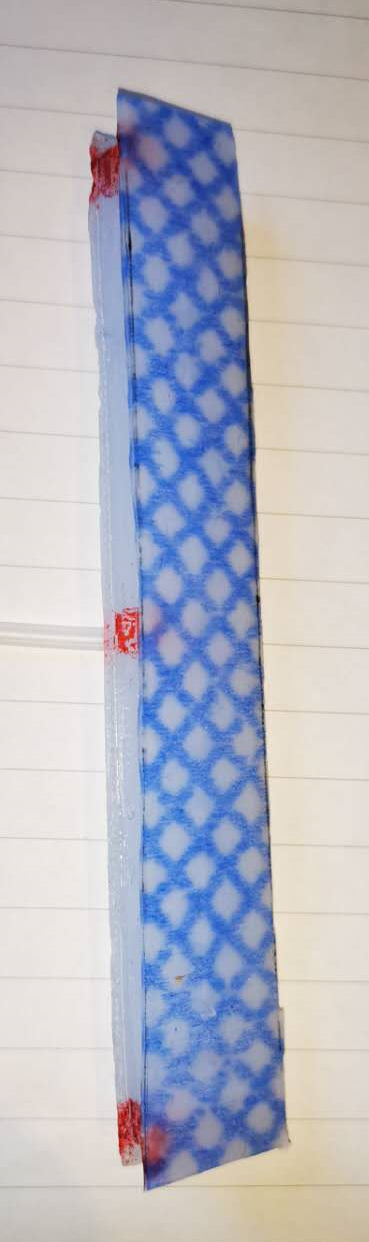
\includegraphics[width=0.15\textwidth]{pics/弹性体示意图.png}
  \caption{Elastomer gripper investigated in this article. The blue grid at the bottom is the strain limited layer.}
\end{wrapfigure}

The materials used for soft robot actuators are typically intrinsically isotropic, which means that their strain characteristics are consistent through their whole body. This property makes it difficult for a soft robot actuator made of a single material to exhibit complex behavior. However, this drawback can be partially overcome by introducing other materials as constraints. Fiber materials, due to their flexibility and softness, as well as the fact that they are a commonly used material, make them suitable materials for introducing anisotropic properties into soft robot actuators \cite{overview}.



% 本文中将对布里斯托大学 MSc Robotics 课程 Soft Rbotics 提供的纤维补强执行器进行研究(此处插入图片解释,全貌,受压力的形变效果)。作为一种用压力限制层(nature那个)来补强的纤维补强弹性体,其压力限制层位于长方体弹性体的一个长侧面上。有趣的是,虽然压力限制层是为了给各向同性的弹性体引入约束使其具有一定程度的各向异性特性,但是课程模组本身所提供的压力限制层(Wilco all purpose cloths)也具有各向异性,其受到水平方向拉力时产生的应变可以分解为两个正交的轴向,在一轴上较易发生轴向的应变,在另一轴上则较不容易发生轴向的应变。这就导向了一个问题:压力限制层的方向会对纤维增强弹性体的应变特性产生什么影响?
This article focuses on the fiber-reinforced gripper provided in the Soft Robotics module of the MSc Robotics program at the University of Bristol (Fig. 1). As a fiber-reinforced elastomer with a strain limited layer\cite{stress_constraint_layer}, the interesting thing is that although the strain limited layer is introduced to provide some degree of anisotropic properties to the isotropic elastomer, the stress limited layer provided in the course module  (Wilco all purpose cloths) itself is also anisotropic. When subjected to a horizontal tensile force, the cloths' strain can be decomposed into two orthogonal axial components, with axial strain being more easily generated in one axis than in the other. This leads to the question: \textbf{how does the direction of the strain limited layer affect the strain characteristics of the fiber-reinforced elastomer?}





\subsection{Hypothesis Statement}
\label{Hypothesis}

% 基于以上描述,本文的假想是:使用各向异性的压力限制层来强化执行器的时候,压力限制层的方向会影响弹性体的应变特性。

Based on the description above , the hypothesis of this study is:
\begin{quote}
\textbf{When using an anisotropic stress limited layer to reinforce the actuator, the orientation of the stress limited layer will affect the strain characteristics of the actuator.}
\end{quote}

% 此设想是受(2)启发,由于纤维补强型执行器的原理就是用纤维的应变特性来限制弹性体某一方向的形变,使其不对称从而对其进行某种物理编程(cite那个通过改变纤维角度对其进行物理编程)。对于本文中所使用的具体执行器来说,就是压力限制层会限制弹性体一侧的变形,从而使得弹性体在受到内部气压的时候向一侧弯曲,从而使其产生适合抓握的形状。如果本文的假设成立的话,此执行器就有可能通过在不同位置将压力限制层的方向对其进行进一步的物理编程,如在特定位置放置关节,使其更适合抓握。

This hypothesis is inspired by \cite{mechanical_programing}, as the principle of fiber-reinforced actuators is to use the strain characteristics of the fibers to limit the deformation of the elastomer in a certain direction, making it asymmetric and allowing for some kind of physical programming \cite{fingerlike}. 

For the specific actuator used in this study, the strain limited layer restricts deformation on the bottom of the elastomer, causing it to bend towards another side when subjected to internal pressure, resulting in a shape suitable for grasping. If the hypothesis of this study is confirmed, it may be possible to further physically program this actuator by varying the direction of the pressure-limiting layer at different positions, such as placing joints in specific locations to make the actuator more suitable for grasping.

% 本文中将会先研究压力限制层不同朝向对弹性体形变的影响,若有可见的影响,则测试此种影响用于物理编程的可能性。

This report will investigate the effect of different orientations of the strain limited layer on the deformation of the elastic body.

% 本文的结构如下:
% 1.介绍:介绍文章的研究背景与假设
% 2.设计与方法论:描述制造的过程以及实验方法论
% 3.结果与分析:描述并分析实验的结果
% 4.讨论:评价试验结果与假设的关系

The structure of this article is as follows:
\begin{enumerate}
    \item \textbf{Introduction}: Introduce the motivation and hypothesis of this article.
    \item \textbf{Design and methods}: Describe the experimental methodology.
    \item \textbf{Results and analysis}: Describe and analyze the results of the experiment.
    \item \textbf{Conclusion}: Limitations and conclusion of this article.
\end{enumerate}


\section{Design and methods}


% 为了对比应变限制层方向对弹性体形变的影响,本文将采用如下所述的方法。
\subsection{Term Definition}
Here are some terms that will be used in this article.
\begin{itemize}
    \item \textbf{Direction} (of the strain limited layer): when the same magnitude of tensile force is applied to the strain limited layer from different directions, the direction that maximizes the strain of the strain limited layer is defined as the direction of the strain limited layer.
    \item \textbf{Standard direction}: pointing from the center of the gripper towards the tip of gripper fingers.
    \item \textbf{Tilt} (of the strain limited layer): the angle between the direction of strain limited layer and the standard direction. The range of tilt is $[0°,90°]$ for the gripper is symmetry.
    \item \textbf{Standard side} (of the gripper): gripper finger with strain limited layer of 0° tilt (as shown in Fig. \ref{fig:Grippers}).
    \item \textbf{Comparing side} (of the gripper): gripper finger with strain limited layer of a certain angle of tilt.
\end{itemize}

\subsection{Overview of Method}

\begin{comment}
    
Describe to the reader the general structure and procedure of your experiment. You should provide a specification a bit like a cake recipe.  For example: how long does your experiment last?  how many repeated trials do you use?  how many alternate scenarios are there?
\end{comment}


% 为了减少实验中大量无关变量的干扰,采用的方法是:在同一抓握器的两个手指上使用不同方向的应变限制层。其中一根手指采用正常的方向(从指根指向指尖),另一根手指的应变限制层则相对正常方向有一定的倾斜。 我制作了三个抓握器,其中一个双指都为标准朝向,一个是标准+45度倾斜的组合,一个是标准+90°倾斜的组合。
To reduce the interference of a large number of irrelevant variables in the experiment, the method employed was to use strain limited layers of different orientations on two fingers of the same gripper. Strain limited layer on one finger is using the standard direction, while the strain limited layer on the other finger is tilted at a certain angle. I made three grippers (as shown in Fig. \ref{fig:Grippers}), one with both fingers in the standard direction, one with a combination of standard direction and a 45° tilt, and one with a combination of standard direction and a 90° tilt. 


% 对上图中的抓握器推入等量的空气,观察标准端和倾斜端的形变,就可以观察到应变限制层倾斜角度对弹性体应变特性的影响。具体流程如下所示:
To observe the effect of the direction of inclination of the strain limited layer on the strain characteristics of the elastomer, equal amounts of air (30ml) were injected into the grippers shown in the Fig. \ref{fig:Grippers}, and the displacement of both the standard side and the comparing side were observed. The specific process is shown as follows:

\begin{algorithm}
\label{Algorithm}
	\caption{Experiment Process}\label{pseudo:ExperimentProcess}
	\begin{algorithmic}[1]
            \State Mark the center and both ends of the gripper in red for tracking.
            \State Place the gripper at the centre of a black square (approximately 14.4$\times$15.7cm) drawn on the paper. The specific orientation for placing the gripper is as shown in Figure \ref{fig:three_images}.
            \State A video of injecting 30 ml of air into the gripper is recorded using a smartphone from a fixed distance and angle.
            \State Eliminate potential errors caused by camera angle by remapping the black square corners to the corners of a 1000$\times$1000 video. 
            \State Find the coordinates of both side ends.
            \State Calculate the horizontal (as shown in Fig. \ref{fig:Displacement}) displacement of the distance between the ends of both sides from the center.
            \State When there is any displacement change on either side, record the displacement values of both sides at that time. Generate a series of displacement data points (data serie shape: $n$ points $\times$ 1 row $\times$ 2 columns). Each point of the data is formatted as: (standard side displacement, comparing side displacement).
            \State Repeat 5 times for each gripper, and save the data for processing detailed in Section \ref{Processing}.
	\end{algorithmic} 
\end{algorithm}



\begin{figure}
    \centering
    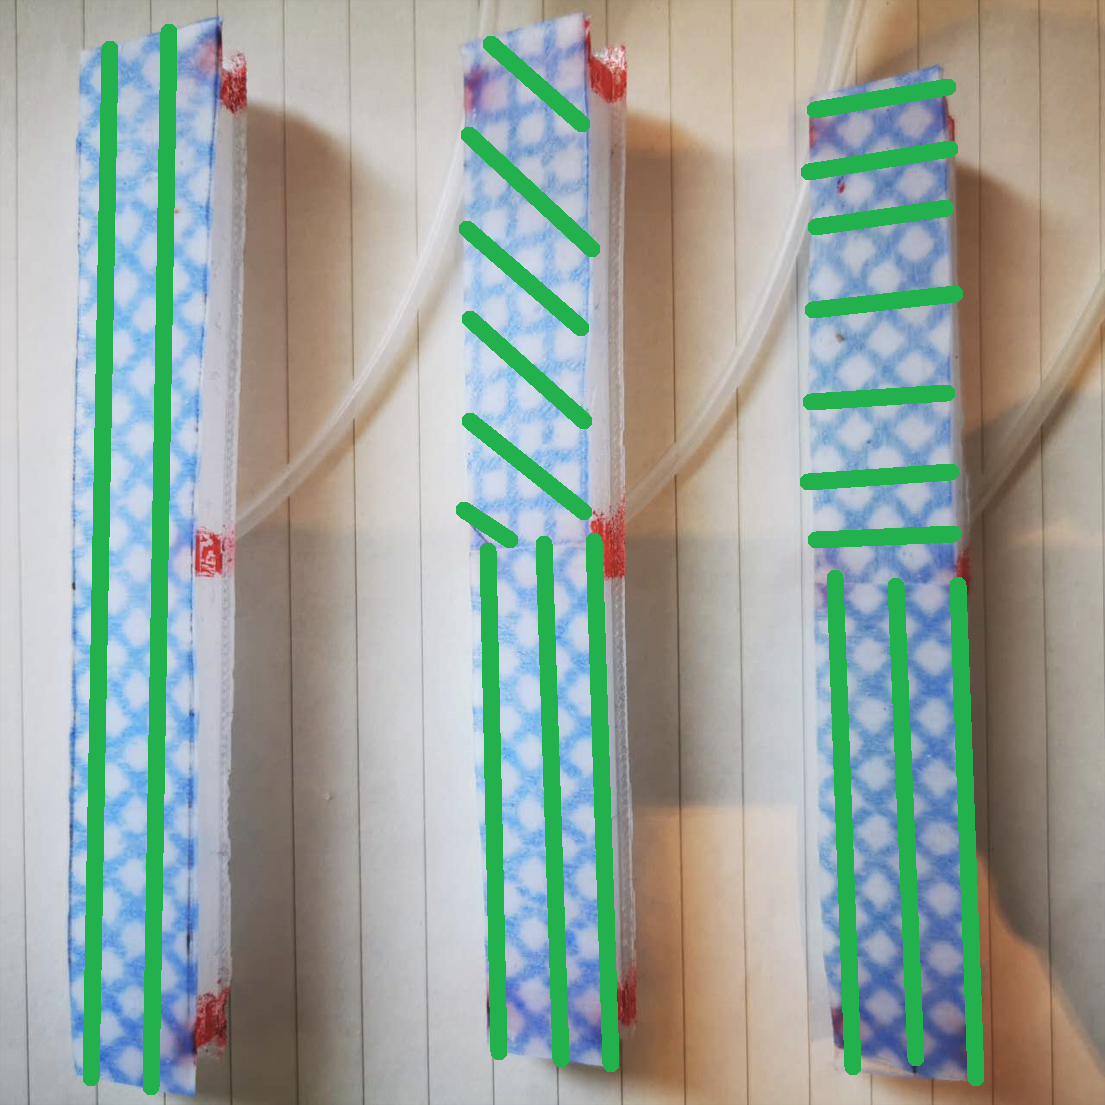
\includegraphics[width = 0.85\linewidth]{pics/实验示意图1.png}
    \caption{Grippers with different directions of strain limited layers. From left to right in the figure, they are: standard, standard $+$ 45° tilt, and standard $+$ 90° tilt. The direction of the red arrows in the figure indicate the directions of the strain limited layer.}
    \label{fig:Grippers}
\end{figure}

\begin{figure}
    \centering
    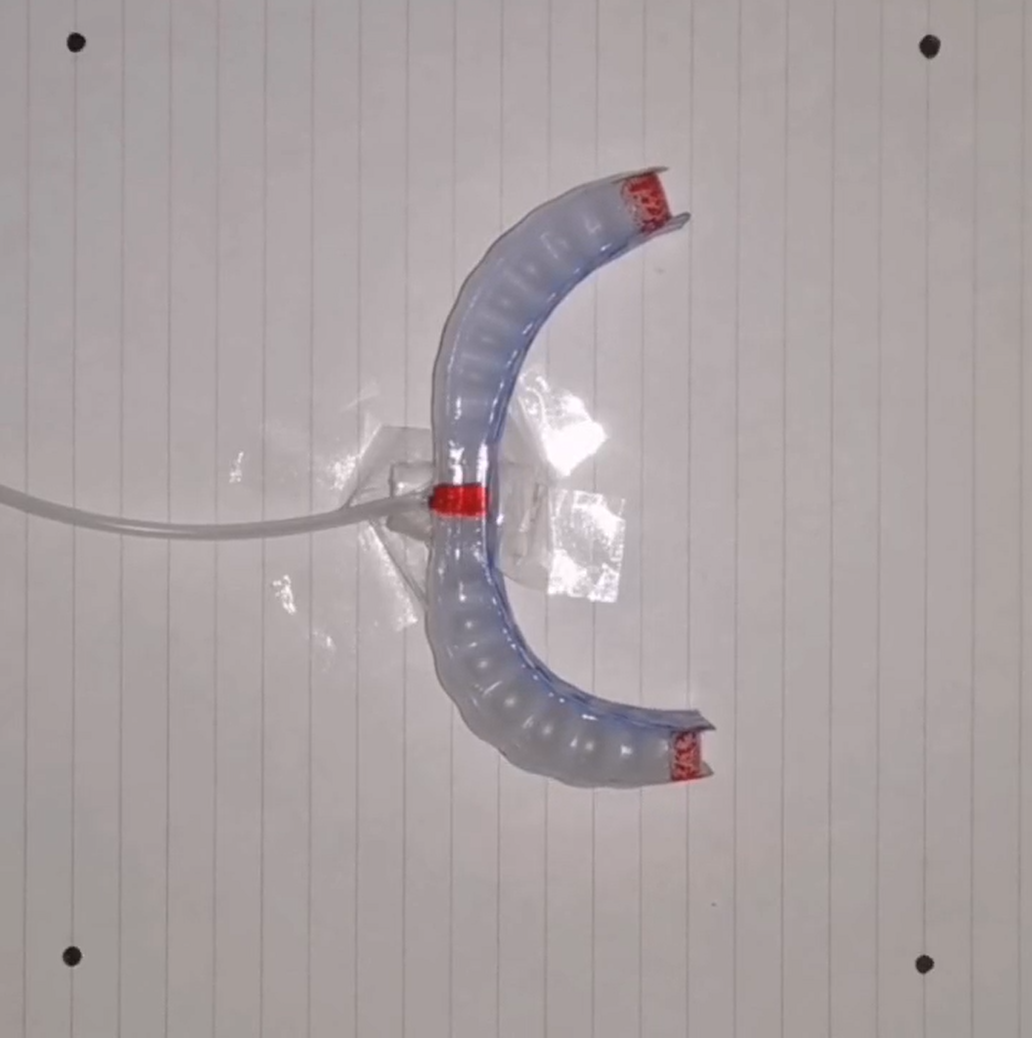
\includegraphics[width = 0.85\linewidth]{pics/位移计量示意图.png}
    \caption{Displacement measurement. For simplicity, only the horizontal (along y-axis of the video) displacement was measured.}
    \label{fig:Displacement}
\end{figure}


\begin{figure}[htbp]
  \centering
  \begin{subfigure}[b]{0.25\linewidth}
    \centering
    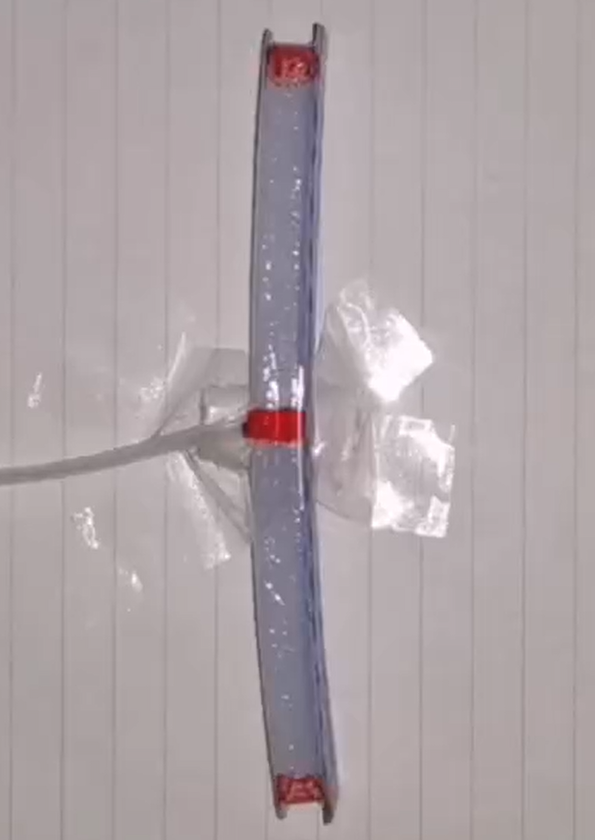
\includegraphics[width=\linewidth]{pics/变形1.png}
    \caption{}
    \label{fig:image1}
  \end{subfigure}
  \begin{subfigure}[b]{0.25\linewidth}
    \centering
    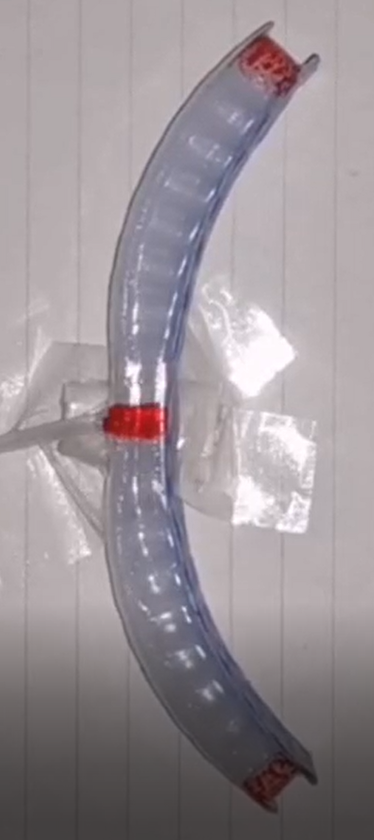
\includegraphics[width=\linewidth]{pics/变形2.png}
    \caption{}
    \label{fig:image2}
  \end{subfigure}
  \begin{subfigure}[b]{0.25\linewidth}
    \centering
    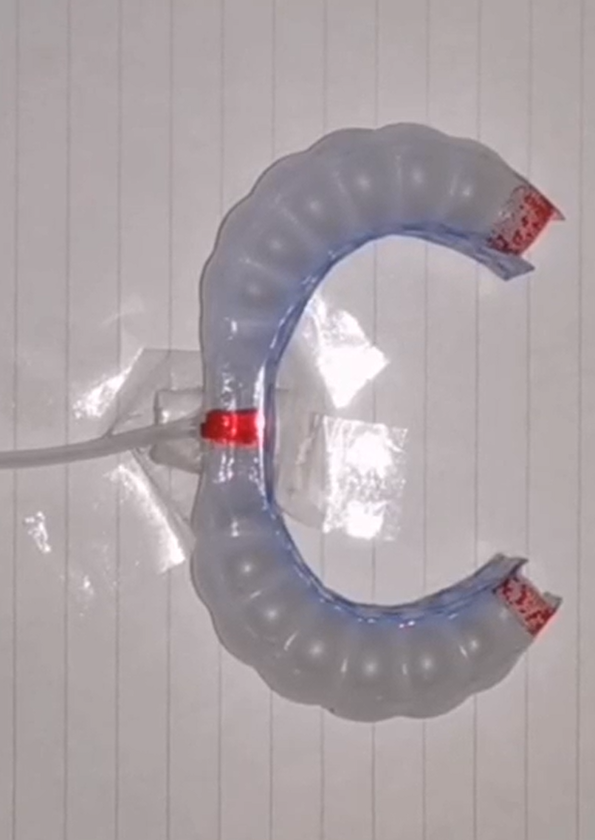
\includegraphics[width=\linewidth]{pics/变形3.png}
    \caption{}
    \label{fig:image3}
  \end{subfigure}
  \caption{Frames from the recorded video. The gripper is bending towards the positive direction of the y-axis of the picture.}
  \label{fig:three_images}
\end{figure}

\subsection{Data Processing}
\label{Processing}

% 实验流程中得到的数据是一连串二维坐标点,格式为:(对比侧应变,标准侧应变)。
% 为了使数据具有可比性,将其平移到(0,0)的原点处
% 由于实验较为简单,其中有较多的干扰,所以数据中的噪声比较严重。后续将在提供原始数据平均值折线图的同时,也提供用三次多项式拟合产生的结果,来更好地展示应变特性的变化。
The data obtained in the experimental procedure is a series of two-dimensional coordinate points, in the format of (standard side displacement, comparing side displacement).

In order to make the data comparable, All data series are shifted to the origin $(0,0)$.

Due to the simplicity of the experiment, there is a lot of interference, resulting in significant noise in the data. In order to better illustrate the variation of strain characteristics, we will provide both the average of the raw data and the results generated by fitting with a fifth-order polynomial in Section \ref{results}.


\subsection{Discussion of Variables}

\begin{itemize}
    \item \textbf{Controlled Variables}: % 注入的空气多少 视频的尺寸 弹性体本身 
    \begin{itemize}
        \item \textbf{Air injected}: Use the markings on the syringe to ensure the injection of 30ml of air for each experiment. 30ml of air is sufficient to cause maximum deformation in all grippers.

\begin{figure*}[htbp]
  \centering
  \begin{minipage}[t]{0.32\textwidth}
    \centering
    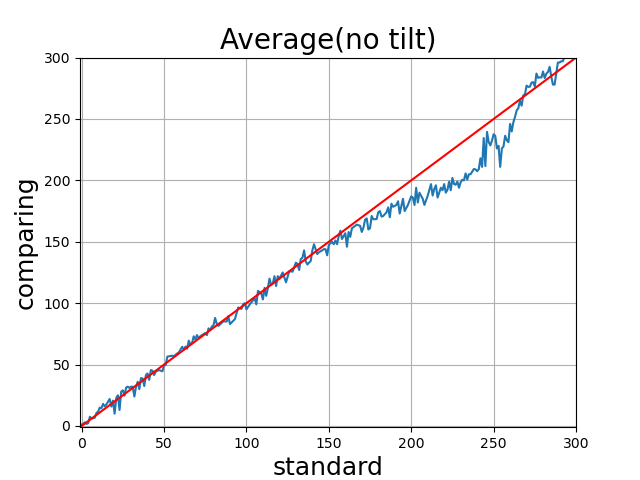
\includegraphics[width=\textwidth]{pics/Section3/Average0.png}

  \end{minipage}
  \hfill
  \begin{minipage}[t]{0.32\textwidth}
    \centering
    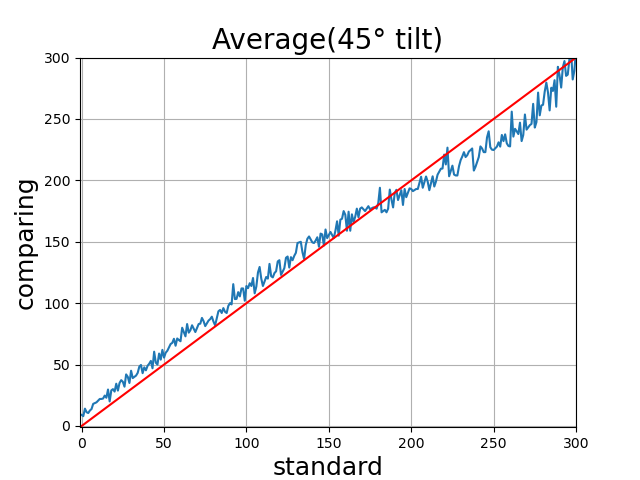
\includegraphics[width=\textwidth]{pics/Section3/Average45.png }

  \end{minipage}
  \hfill
  \begin{minipage}[t]{0.32\textwidth}
    \centering
    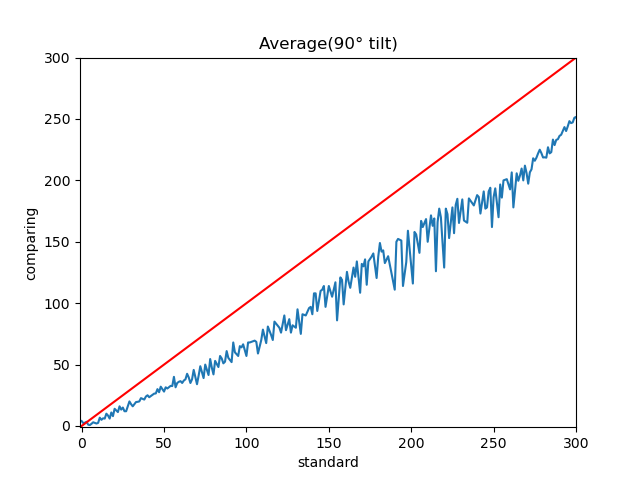
\includegraphics[width=\textwidth]{pics/Section3/Average90.png}

  \end{minipage}

  \vspace{1em}

  \begin{minipage}[t]{0.32\textwidth}
    \centering
    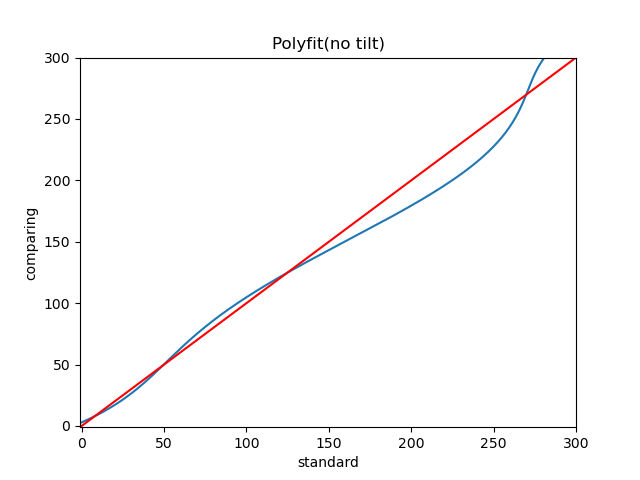
\includegraphics[width=\textwidth]{pics/Section3/Polyfit0.png}

  \end{minipage}
  \hfill
  \begin{minipage}[t]{0.32\textwidth}
    \centering
    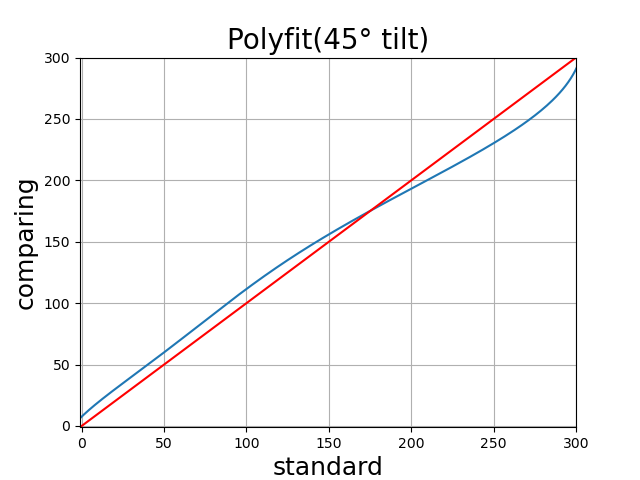
\includegraphics[width=\textwidth]{pics/Section3/Polyfit45.png}

  \end{minipage}
  \hfill
  \begin{minipage}[t]{0.32\textwidth}
    \centering
    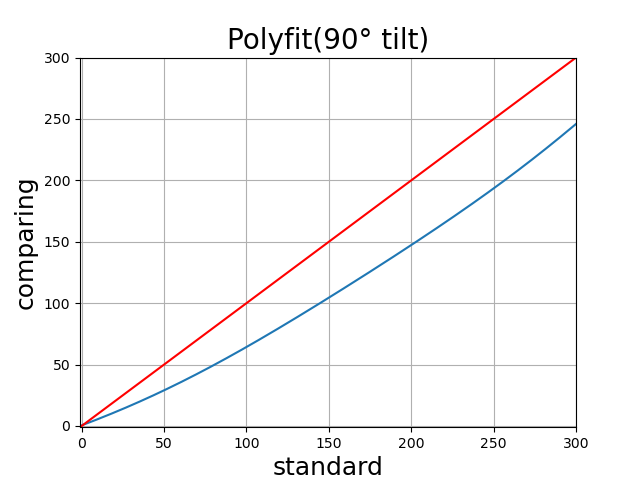
\includegraphics[width=\textwidth]{pics/Section3/Polyfit90.png}
  \end{minipage}
  
  \caption{Overview of experiment results: Axes in all pictures are gripper finger strain in pixels. The top row shows the average value of the five repeating experiments, and the bottom row shows the average of five fifth-order polynomials, each of the polynomials was fitted with one of the five repeating experiments. Red lines are 45° lines.}
  \label{fig:OverallResult}


\end{figure*}

%\FloatBarrier

        
        \item \textbf{Video size}: Always remap the black square to the size of 1000$\times$1000 pixels. This made the actual size of the black square irrelevant to the experiment, because I'm using the same square across the whole experiment, and it is always remapped to the same size.
        \item \textbf{Gripper}: Use the same mold to make elastomers, try to make the grippers as identical as possible. However, due to limitations in the fabrication environment, this variable is not guaranteed to be fully controlled.
        \item \textbf{Inner Pressure}: For each data point, the comparing displacement and standard displacement are caused by the same level of inner pressure for they are fingers of the same gripper.
        \item Direction of strain limited layer on \textbf{standard side}:  As previously shown in Fig. \ref{fig:Grippers}, the direction of the strain limited layers on the standard sides is identical (0° tilt).
    \end{itemize}



    \item \textbf{Independent Variable}: 
        \begin{itemize}
            \item Direction of strain limited layer on \textbf{comparing side}: As previously shown in Fig. \ref{fig:Grippers}, the direction of the strain limited layers on the comparing sides is the independent variable. 
        \end{itemize}
    \item \textbf{Dependent Variable(s)}: 
         \begin{itemize}
             \item Displacement of the tip of comparing side (as shown in Fig. \ref{fig:Displacement}).
             \item Displacement of the tip of standard side.
             \item The relationship between the displacement of the standard side tip and the displacement of the comparing side tip.
         \end{itemize}
\end{itemize}

\subsection{Discussion of Metric}

\begin{comment}
 In this section you should discuss the rationale (why) you have selected your metric(s) - e.g. how do these metrics help us to interpret your results?  Your metric(s) will need to be applied consistently throughout your experiment for them to provide a comparison of performance.  
 
 You should discuss the advantages and disadvantages of your metric(s).  Often, we need more than one metric to compensate for the information which is confused or hidden in another metric.  By using more than one metric, we can get closer to the truth of the outcome of your experiment.  
\end{comment}

% 如前所述,本实验最后会对每一个标准侧形变值获得一个对应的同等充气程度(同等压力)下的对比侧形变值。
As previously mentioned, the experiment will obtain a series of corresponding displacement value of the comparing side for each displacement value of the standard side. Each pair of the displacement values are results of the same inner pressure.

% 只要对于每一个标准侧位移值比较其对应的几个不同的对比侧位移值的大小,就可以简单地看出不同对比侧应变特性的区别。
 Simply by comparing different corresponding displacement values of the comparing side for each standard side displacement value, the differences in strain characteristics of different comparing sides can be easily observed.

 % 此metrics的好处在于,可以直观地观察出对比侧的“硬度”,
 % 不同抓握器之间的区别不会对结果有较大影响,因为对比是对比同一个标准侧位移值对应的多个对比侧位移值,实际上是用内部压力的作用结果来进行比较。由于抓握器的制作比较简单,无法保证抓握器之间的一致性,如有些抓握器腔壁比较厚,其应变特性就会改变,这时用内部压力作为指标的一部分就会不公平。
 % 此metrics的坏处在于,不能排除同一抓握器两根手指之间的区别造成的干扰。
 \textbf{Advantages}:
 \begin{itemize}
     \item The 'hardness' of different comparing sides could be easily observed. 
     \item The differences between different grippers will not have a significant impact on the results. This metric concerns displacement only, and its fair to all grippers, even the grippers could be slightly different from each other.
 \end{itemize}
 
 \textbf{Disadvantages}:
  \begin{itemize}
     \item Cannot exclude the interference caused by differences between the two fingers of the same gripper. If one finger is more "softer" than another (as shown in Fig. \ref{fig:flawed}), the experiment result will be significantly affected.
 \end{itemize}




\section{Results and Analysis}

\label{results}

% 图3中展示了实验的总体结果。
% 图3中,每一个点都代表标准侧应变所对应的一个对比侧应变。图中的横轴和纵轴单位均为像素。
% 图中红色斜线为45°直线,用于直观地看出应变特性的变化。
% 曲线位于红线上则代表抓握器的两侧应变特性相似。位于红线下则代表对比侧比标准侧更不容易发生位移,位于红线上则代表对比侧比标准侧更易发生形变。
\subsection{Graph explanation}


Fig. \ref{fig:OverallResult} shows the overall results of the experiment. For all graphs in Fig. \ref{fig:OverallResult}, the axes are comparing side displacement and standard side displacement, and the unit for both axes are pixels.

The reason for cutting off both of the axes at value 300 is that, according to observation, the maximum displacement of the gripper in this experiment is about 320 pixels. After removing the unstable portion of the data at the end, it was found to be at 300 pixels.



The red diagonal line in the figure is the 45° line, which is used to visually illustrate the variation in strain characteristics. 
\begin{itemize}
    \item If the curve that lies \textbf{on the red line}, it indicates that the strain characteristics on both sides of the gripper are \textbf{similar}. 
    \item If the curve lies \textbf{below the red line}, it indicates that \textbf{the comparing side is less likely to strain} than the standard side.
    \item If the curve lies \textbf{above the red line}, it indicates that \textbf{the comparing side is more likely to strain} than the standard side.
\end{itemize}


\subsection{Result Analysis}
\label{Analysis}

\begin{figure}
    \centering
    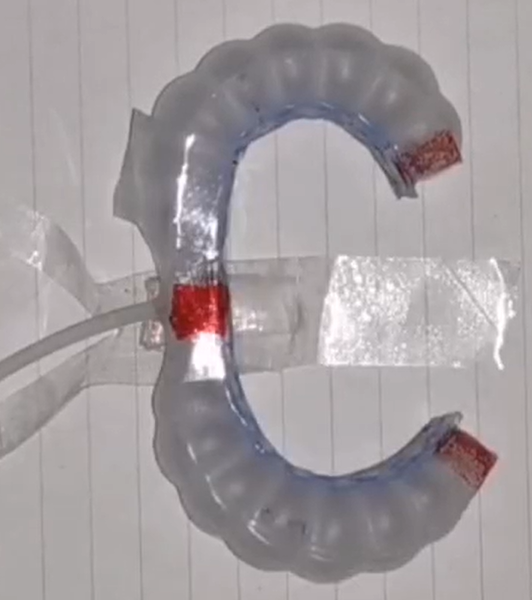
\includegraphics[width = 0.3\linewidth]{pics/Section3/Trivial.png}
    \caption{A fully stretched gripper with 90° tilted strain limited layer. The effect on the strain characteristic is trivial.}
    \label{fig:Trivial}
\end{figure}

\subsubsection{About the Hypothesis}
\begin{itemize}
    \item \textbf{Results support the hypothesis}: From Fig. \ref{fig:OverallResult}, the strain characteristic is changed as the strain limited layer direction changes. This phenomenon supports the hypothesis purposed in Section \ref{Hypothesis}. 
    \item \textbf{Tilt angle vs Strain characteristic}: 90° tilt shown greatest effect and the effect of 45° tilt was smaller, which possibly indicates that the more the strain limited layer is tilted towards 90° (which is vertical to the strain direction), the more significant its effect on the strain characteristics. The more the strain limiting layer tilts, the harder for the gripper fingers to undergo strain (require higher pressure for the same level of strain). 
    \item \textbf{Level of effect}: Although the effect of strain limited layer is clear in the Fig. \ref{fig:OverallResult}, its effect on the strain is trivial (as shown in Fig. \ref{fig:Trivial}), which means its potential for physically programming is limited.
\end{itemize}

\subsubsection{Other than the Hypothesis}
\label{OtherThanTheHypothesis}

\begin{itemize}
    \item  \textbf{Noise in the average curve}: The average data curve has sustained small fluctuations while the overall trend is unaffected. Its the zeroing (see Section \ref{Processing}) that is causing this. Though all data were shifted to make their origin at (0,0), but these data are not actually started from the same origin, its because the physically zeroing of the gripper is not precise. This has no effect on the general trend of the curve.
    \item \textbf{Other factors that affects the strain characteristic}: The manufacturing of the gripper could be divided into two stages: casting (casting the elastomer) and bonding (attaching the strain limited layer). Flaws in each of these stages could have significant influence on the strain characteristic.
        \begin{itemize}
            \item Casting stage flaw (Fig. \ref{fig:uneven}): If some chambers have thinner walls than the others, they would be much more easier to expand and will significantly affect the strain characteristic.
            \item Bonding stage flaw (Fig. \ref{fig:notattached}): If some of the chamber walls are not attached to the strain limited layer, causing two chambers partially merged into one, the merged chambers are also easier to strain and the strain characteristic would be significantly affected.
        \end{itemize}
        Though these two factors have great impact on the strain characteristic, they are not controllable with the toolbox given. So they are considered as interferences to the experiment, and all grippers used in experiment are grippers without significant flaws.
\end{itemize}


\begin{figure}[htbp]
\centering
\begin{minipage}[t]{0.48\linewidth}
\centering
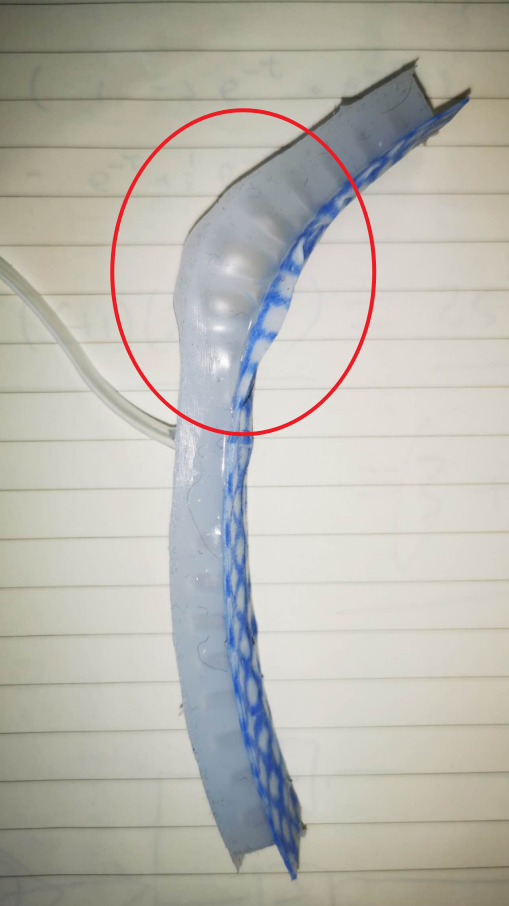
\includegraphics[width=0.8\linewidth]{pics/Section3/uneven.png}
\subcaption{Gripper with uneven chamber walls.}
\label{fig:uneven}
\end{minipage}
\begin{minipage}[t]{0.48\linewidth}
\centering
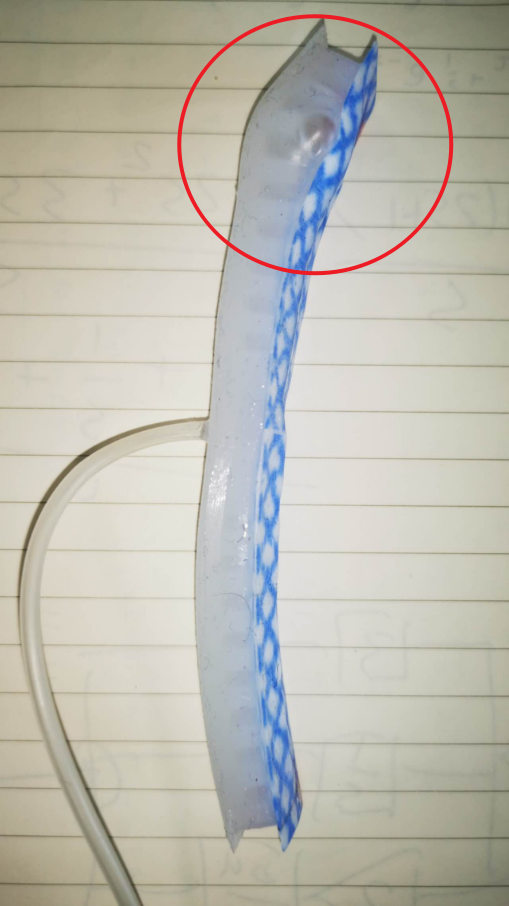
\includegraphics[width=0.8\linewidth]{pics/Section3/notattached.png}
\subcaption{Gripper with chamber walls not attached to the cloth.}
\label{fig:notattached}
\end{minipage}
\caption{Flawed grippers. Flaws are marked with red circles.}
\label{fig:flawed}
\end{figure}




\section{Conclusion}

\label{DiscussionAnConclusion}

\subsection{Discussion on the results}

Because the strain limited layer provided in the module has anisotropic strain characteristic, we hypothesised in Section \ref{Hypothesis} that:

\begin{quote}
When using an anisotropic stress limited layer to reinforce the actuator, the direction of the stress limited layer will affect the strain characteristics of the actuator.
\end{quote}

\begin{comment}
Make a discussion of what your results showed - whether this supported or refuted your hypothesis.  It may be that the results were mixed (supporting and refuting) and you should discuss that here. In your discussion, use this as another opportunity to demonstrate/evidence your understanding. Try to avoid stating the obvious - instead, use analysis/evaluation/synthesis to show that you understand \emph{how} and \emph{why} you saw the results you did.  What are the implications of your findings?  
This is also a good opportunity to evaluate your experiment and project as a whole.  You may wish to further discuss the limitations of the study (e.g. the difficulty of controlled/dependent variables, or any problems you faced in your project).  You may wish to make a recommendation for future work - but ensure that this is a clear advancement from the understanding you have gained and not wild speculation.
\end{comment}

Results shown in Fig. \ref{fig:OverallResult} supports the hypothesis. 

By tilting the strain limited layer, the strain characteristic of the gripper could be changed, and the more the strain limited layer tilts toward 90°, the more significant the effect is. But the effect is trivial and may not be a practical way to physically programming the gripper.


There are also other factors (see Section \ref{OtherThanTheHypothesis}) that have much more significant effect on the gripper's strain characteristic, but they are not controllable with the tools provided and are treated as interferences to the experiment.

\subsection{Limitations}
% 无法消除的干扰
\begin{itemize}
    \item Several interferences that cannot be eliminated: There are several variables that I didn't figure a way to control: differences between two fingers of the same gripper, zeroing of the gripper fingers (grippers have permanent deformation after each inflation). Effects of these factors cannot be ignored, and I tried my best to reduce the impact of these interferences by operating the experiment carefully, but perfect consistency cannot be achieved manually.
    \item Limitation of the material: The material provided is limited and cannot conduct experiments in larger scale with that. The experiment could be operated on more grippers and more strain limited layer directions.
\end{itemize}
% 受试角度有限
% 

\subsection{Conclusion}

The direction of the anisotropic stress limited layer could have effect on the strain characteristic on the gripper, and the degree of effect is related with the direction. But this effect is trivial and cannot be used for physical programming on its own. 




\bibliographystyle{ieeetr} 
\bibliography{ref}


\end{document}
